\documentclass{standalone}
\usepackage{tikz}
\usetikzlibrary{patterns, positioning}


\begin{document}
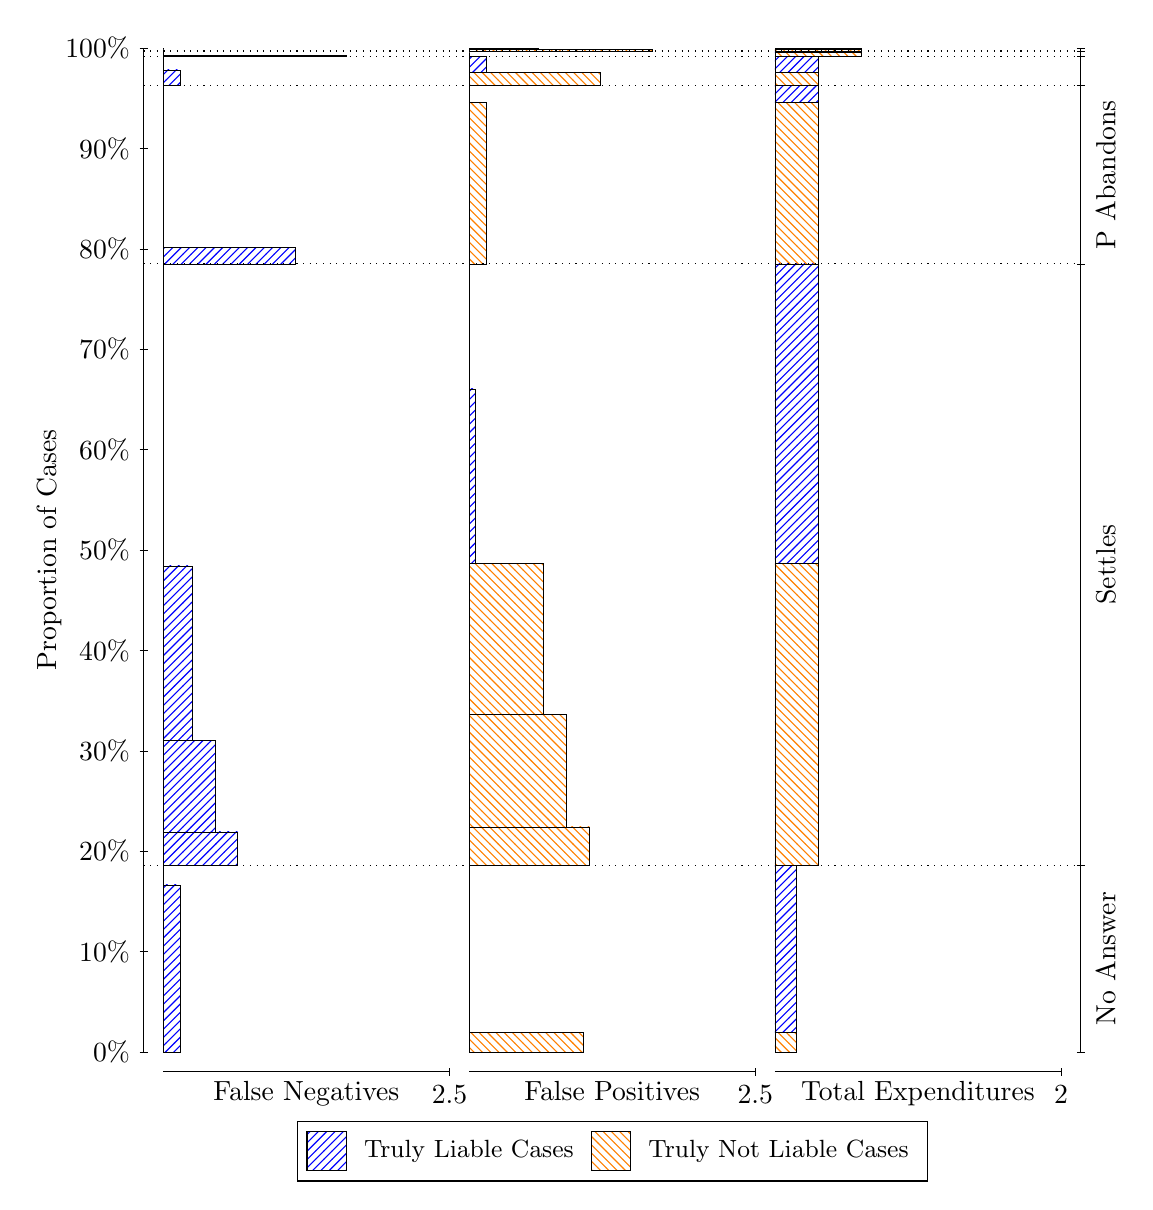
\begin{tikzpicture}
\draw[black, very thin] (1.5,1.75) -- (1.5,14.5);
\node[rotate=90, text=black, anchor=center] at (0.3, 8.125) {Proportion of Cases};
\draw[black, very thin] (1.45,1.75) -- (1.55,1.75);
\node[text=black, anchor=east] at (1.45, 1.75) {0\%};
\draw[black, very thin] (1.45,3.025) -- (1.55,3.025);
\node[text=black, anchor=east] at (1.45, 3.025) {10\%};
\draw[black, very thin] (1.45,4.3) -- (1.55,4.3);
\node[text=black, anchor=east] at (1.45, 4.3) {20\%};
\draw[black, very thin] (1.45,5.575) -- (1.55,5.575);
\node[text=black, anchor=east] at (1.45, 5.575) {30\%};
\draw[black, very thin] (1.45,6.85) -- (1.55,6.85);
\node[text=black, anchor=east] at (1.45, 6.85) {40\%};
\draw[black, very thin] (1.45,8.125) -- (1.55,8.125);
\node[text=black, anchor=east] at (1.45, 8.125) {50\%};
\draw[black, very thin] (1.45,9.4) -- (1.55,9.4);
\node[text=black, anchor=east] at (1.45, 9.4) {60\%};
\draw[black, very thin] (1.45,10.675) -- (1.55,10.675);
\node[text=black, anchor=east] at (1.45, 10.675) {70\%};
\draw[black, very thin] (1.45,11.95) -- (1.55,11.95);
\node[text=black, anchor=east] at (1.45, 11.95) {80\%};
\draw[black, very thin] (1.45,13.225) -- (1.55,13.225);
\node[text=black, anchor=east] at (1.45, 13.225) {90\%};
\draw[black, very thin] (1.45,14.5) -- (1.55,14.5);
\node[text=black, anchor=east] at (1.45, 14.5) {100\%};

\draw[black, very thin] (13.4,1.75) -- (13.4,14.5);
\draw[black, very thin] (13.35,1.75) -- (13.45,1.75);
\node[anchor=west] at (13.35, 1.75) {};
\draw[black, very thin] (13.35,4.1222) -- (13.45,4.1222);
\node[anchor=west] at (13.35, 4.1222) {};
\draw[black, very thin] (13.35,11.76) -- (13.45,11.76);
\node[anchor=west] at (13.35, 11.76) {};
\draw[black, very thin] (13.35,14.022) -- (13.45,14.022);
\node[anchor=west] at (13.35, 14.022) {};
\draw[black, very thin] (13.35,14.389) -- (13.45,14.389);
\node[anchor=west] at (13.35, 14.389) {};
\draw[black, very thin] (13.35,14.462) -- (13.45,14.462);
\node[anchor=west] at (13.35, 14.462) {};
\draw[black, very thin] (13.35,14.5) -- (13.45,14.5);
\node[anchor=west] at (13.35, 14.5) {};

\draw[black, very thin, pattern color=blue, pattern=north east lines] (1.75,1.75) rectangle (1.968,3.8726);
\draw[black, very thin, pattern color=orange, pattern=north west lines] (1.75,3.8726) rectangle (1.75,4.1222);
\draw[black, very thin, pattern color=blue, pattern=north east lines] (1.75,4.1222) rectangle (2.6947,4.5456);
\draw[black, very thin, pattern color=blue, pattern=north east lines] (1.75,4.5456) rectangle (2.404,5.711);
\draw[black, very thin, pattern color=blue, pattern=north east lines] (1.75,5.711) rectangle (2.1133,7.9234);
\draw[black, very thin, pattern color=orange, pattern=north west lines] (1.75,7.9234) rectangle (1.75,11.76);
\draw[black, very thin, pattern color=blue, pattern=north east lines] (1.75,11.76) rectangle (3.4213,11.972);
\draw[black, very thin, pattern color=orange, pattern=north west lines] (1.75,11.972) rectangle (1.75,14.022);
\draw[black, very thin, pattern color=blue, pattern=north east lines] (1.75,14.022) rectangle (1.968,14.223);
\draw[black, very thin, pattern color=orange, pattern=north west lines] (1.75,14.223) rectangle (1.75,14.389);
\draw[black, very thin, pattern color=blue, pattern=north east lines] (1.75,14.389) rectangle (4.0753,14.408);
\draw[black, very thin, pattern color=orange, pattern=north west lines] (1.75,14.408) rectangle (1.75,14.462);
\draw[black, very thin, pattern color=orange, pattern=north west lines] (1.75,14.462) rectangle (1.75,14.481);
\draw[black, very thin, pattern color=blue, pattern=north east lines] (1.75,14.481) rectangle (1.75,14.5);
\draw[black, very thin, pattern color=orange, pattern=north west lines] (5.6333,1.75) rectangle (7.0867,1.9996);
\draw[black, very thin, pattern color=blue, pattern=north east lines] (5.6333,1.9996) rectangle (5.6333,4.1222);
\draw[black, very thin, pattern color=orange, pattern=north west lines] (5.6333,4.1222) rectangle (7.1593,4.6075);
\draw[black, very thin, pattern color=orange, pattern=north west lines] (5.6333,4.6075) rectangle (6.8687,6.0418);
\draw[black, very thin, pattern color=orange, pattern=north west lines] (5.6333,6.0418) rectangle (6.578,7.9586);
\draw[black, very thin, pattern color=blue, pattern=north east lines] (5.6333,7.9586) rectangle (5.706,10.171);
\draw[black, very thin, pattern color=blue, pattern=north east lines] (5.6333,10.171) rectangle (5.6333,11.76);
\draw[black, very thin, pattern color=orange, pattern=north west lines] (5.6333,11.76) rectangle (5.8513,13.81);
\draw[black, very thin, pattern color=blue, pattern=north east lines] (5.6333,13.81) rectangle (5.6333,14.022);
\draw[black, very thin, pattern color=orange, pattern=north west lines] (5.6333,14.022) rectangle (7.3047,14.188);
\draw[black, very thin, pattern color=blue, pattern=north east lines] (5.6333,14.188) rectangle (5.8513,14.389);
\draw[black, very thin, pattern color=orange, pattern=north west lines] (5.6333,14.389) rectangle (5.6333,14.444);
\draw[black, very thin, pattern color=blue, pattern=north east lines] (5.6333,14.444) rectangle (5.6333,14.462);
\draw[black, very thin, pattern color=orange, pattern=north west lines] (5.6333,14.462) rectangle (7.9587,14.481);
\draw[black, very thin, pattern color=blue, pattern=north east lines] (5.6333,14.481) rectangle (6.5053,14.5);
\draw[black, very thin, pattern color=orange, pattern=north west lines] (9.5167,1.75) rectangle (9.7892,1.9996);
\draw[black, very thin, pattern color=blue, pattern=north east lines] (9.5167,1.9996) rectangle (9.7892,4.1222);
\draw[black, very thin, pattern color=orange, pattern=north west lines] (9.5167,4.1222) rectangle (10.062,7.9586);
\draw[black, very thin, pattern color=blue, pattern=north east lines] (9.5167,7.9586) rectangle (10.062,11.76);
\draw[black, very thin, pattern color=orange, pattern=north west lines] (9.5167,11.76) rectangle (10.062,13.81);
\draw[black, very thin, pattern color=blue, pattern=north east lines] (9.5167,13.81) rectangle (10.062,14.022);
\draw[black, very thin, pattern color=orange, pattern=north west lines] (9.5167,14.022) rectangle (10.062,14.188);
\draw[black, very thin, pattern color=blue, pattern=north east lines] (9.5167,14.188) rectangle (10.062,14.389);
\draw[black, very thin, pattern color=orange, pattern=north west lines] (9.5167,14.389) rectangle (10.607,14.444);
\draw[black, very thin, pattern color=blue, pattern=north east lines] (9.5167,14.444) rectangle (10.607,14.462);
\draw[black, very thin, pattern color=orange, pattern=north west lines] (9.5167,14.462) rectangle (10.607,14.481);
\draw[black, very thin, pattern color=blue, pattern=north east lines] (9.5167,14.481) rectangle (10.607,14.5);
\draw[black, dotted] (1.5,4.1222) -- (13.4,4.1222);
\draw[black, dotted] (1.5,11.76) -- (13.4,11.76);
\draw[black, dotted] (1.5,14.022) -- (13.4,14.022);
\draw[black, dotted] (1.5,14.389) -- (13.4,14.389);
\draw[black, dotted] (1.5,14.462) -- (13.4,14.462);
\draw[black, very thin] (1.75,1.5) -- (5.3833,1.5);
\node[text=black, anchor=north] at (3.5667, 1.5) {False Negatives};
\draw[black, very thin] (5.3833,1.45) -- (5.3833,1.55);
\node[text=black, anchor=north] at (5.3833, 1.45) {2.5};

\draw[black, very thin] (5.6333,1.5) -- (9.2667,1.5);
\node[text=black, anchor=north] at (7.45, 1.5) {False Positives};
\draw[black, very thin] (9.2667,1.45) -- (9.2667,1.55);
\node[text=black, anchor=north] at (9.2667, 1.45) {2.5};

\draw[black, very thin] (9.5167,1.5) -- (13.15,1.5);
\node[text=black, anchor=north] at (11.333, 1.5) {Total Expenditures};
\draw[black, very thin] (13.15,1.45) -- (13.15,1.55);
\node[text=black, anchor=north] at (13.15, 1.45) {2};

\node[text=black, centered, rotate=90] at (13.72, 2.9361) {No Answer};
\node[text=black, centered, rotate=90] at (13.72, 7.941) {Settles};
\node[text=black, centered, rotate=90] at (13.72, 12.891) {P Abandons};




\draw (7.449999999999999,1.5) node[draw=none] (baseCoordinate) {};
\begin{scope}[align=center]
        \matrix[scale=0.5, draw=black, below=0.5cm of baseCoordinate, nodes={draw}, column sep=0.1cm]{
            \node[rectangle, draw, minimum width=0.5cm, minimum height=0.5cm, pattern color=blue, pattern=north east lines] {}; &
            \node[draw=none, font=\small, text=black] (B) {Truly Liable Cases}; &
            \node[rectangle, draw, minimum width=0.5cm, minimum height=0.5cm, pattern color=orange, pattern=north west lines] {}; &
            \node[draw=none, font=\small, text=black] (B) {Truly Not Liable Cases}; \\
            };
\end{scope}

\end{tikzpicture}
\end{document}